\chapter{User Manual}

It is easy to get start using Buffalo. I assume you are reasonably familiar with the Visual Studio IDE and the general layout of a VS solution. I also assume you know how to compile a solution and where to find the compiled assembly. Buffalo is developed in VS2012, it is recommended you have the same version of the IDE installed.

\section{Compiling}
To begin, first download the full source code from https://github.com/wliao008/buffalo. Open buffalo.sln in VS2012 and compile the source code. This will produce the Buffalo.dll and BuffaloAOP.exe in their respective bin/debug folder.

For this example we will perform the weaving from a command prompt. So create a folder name under the C drive, here I will call it "Buffalo". Copy Buffalo.dll, BuffaloAOP.exe and Mono.Cecil.dll to C:\textbackslash{Buffalo}. Note this folder can be located anywhere in your system, I am just putting it on the C drive for simplicity.

Now let us create an aspect.

\section{Simple Profiler}
In this example we will create a profiler for our application. Suppose we have the following simple program.

\begin{lstlisting}[caption={Hello program}, label=helloprogram, frame=tb, basicstyle=\scriptsize]
using System;

namespace Hello
{
    class Program
    {
        static void Main(string[] args)
        {
            Hello h = new Hello();
            h.SayHello();
            h.Say("Hey Buffalo how's it going!");

            //pause the console
            Console.Read();
        }
    }

    public class Hello
    {
        public void SayHello()
        {
            Console.WriteLine("Hello World!");
        }

        public void Say(string msg)
        {
            Console.WriteLine(msg);
        }
    }
}
\end{lstlisting}

When the program runs, it will display the following output:
\begin{lstlisting}[caption={Hello program output}, label=helloout, frame=tb, basicstyle=\scriptsize]
Hello World!
Hey Buffalo how's it going!
\end{lstlisting}

And suppose that we want to monitor the program, we want to know when a method was accessed and exited. We can easily create a aspect to do such work.

\begin{lstlisting}[caption={TraceAspect}, label=traceaspect, frame=tb, basicstyle=\scriptsize]
using Buffalo;
using System;

public class TraceAspect : MethodBoundaryAspect
{
    public override void Before(MethodArgs args)
    {
        Display("ENTERING", args);
    }

    public override void After(MethodArgs args)
    {
        Display("EXITING", args);
    }

    public override void Success(MethodArgs args)
    {
        Display("SUCCESSFULLY EXECUTED", args);
    }

    public override void Exception(MethodArgs args)
    {
        Display("EXCEPTION ON", args);
    }

    void Display(string title, MethodArgs args)
    {
        Console.WriteLine("{0} {1}", title, args.FullName);
        foreach (var p in args.Parameters)
        {
            Console.WriteLine("\t{0} ({1}) = {2}", p.Name, p.Type, p.Value);
        }
    }
}
\end{lstlisting}

With the aspect defined, now we can apply this aspect on any of the three different levels. Lets apply it to the Hello class for example.
\begin{lstlisting}[caption={Apply Aspect to the Hello Class}, label=helloaspect, frame=tb, basicstyle=\scriptsize]
[TraceAspect]
public class Hello
{
	//...
}
\end{lstlisting}

Now everything is in place. We can now invoke the BuffaloAOP.exe to perform the weaving. Open a command prompt and navigate to C:\textbackslash{Buffalo}. And issue this command:

\begin{lstlisting}[caption={Invoking BuffaloAOP.exe}, label=buffalocmd, frame=tb, basicstyle=\scriptsize]
C:\Buffalo>BuffaloAOP.exe <path_to_the_hello_program_exe>
\end{lstlisting}

Replace path to the hello program exe with the actual complete path to the program assembly. Suppose the program assembly is located at C:\textbackslash{Projects}\textbackslash{Hello}\textbackslash{bin}\textbackslash{Hello.exe}, we would issue the command as follow:

\begin{lstlisting}[caption={Invoking BuffaloAOP.exe Example}, label=buffalocmd2, frame=tb, basicstyle=\scriptsize]
C:\Buffalo>BuffaloAOP.exe C:\Projects\Hello\bin\Hello.exe
\end{lstlisting}

If everything goes well BuffaloAOP.exe will perform the injection and put the final assembly in the Modified folder inside the folder of the target assembly. In this case it will be at C:\textbackslash{Projects}\textbackslash{Hello}\textbackslash{bin}\textbackslash{Modified}\textbackslash{Hello.exe}. Now when the program runs, it will display the following output:

\begin{lstlisting}[caption={TraceAspect output}, label=traceaspectout, frame=tb, basicstyle=\scriptsize]
ENTERING System.Void Hello.Program::Main(System.String[])
        args (System.String[]) = System.String[]
ENTERING System.Void Hello.Hello::.ctor()
SUCCESSFULLY EXECUTED System.Void Hello.Hello::.ctor()
EXITING System.Void Hello.Hello::.ctor()
ENTERING System.Void Hello.Hello::SayHello()
Hello World!
SUCCESSFULLY EXECUTED System.Void Hello.Hello::SayHello()
EXITING System.Void Hello.Hello::SayHello()
ENTERING System.Void Hello.Hello::Say(System.String)
        msg (System.String) = Hey Buffalo how's it going!
Hey Buffalo how's it going!
SUCCESSFULLY EXECUTED System.Void Hello.Hello::Say(System.String)
        msg (System.String) = Hey Buffalo how's it going!
EXITING System.Void Hello.Hello::Say(System.String)
        msg (System.String) = Hey Buffalo how's it going!
\end{lstlisting}

Line 7 and 12 are the original method output, the rest are the output of the various interception points. Note that line 11 also capture the parameter value passed into each method and is available from the aspect.

\section{Integrate With MS-Build System}

Buffalo can be integrated with MS-Build, so weaving can be invoked automatically when a project is compiled from the Visual Studio IDE. Note that the following instructions are just the bare minimum to get this working, a lot of bell and whistle are omitted.

MS-Build is integrated with Visual Studio IDE via configuration file. For example, a C\# project has the associated .csproj, if open in a text editor you will see a line that reference a different configuration file: Microsoft.CSharp.targets. This file in term reference Microsoft.Common.targets.

Each .NET version has a Microsoft.Common.targets file. Depending on the version you are using, open up this file in a text editor. For example, for .NET 4.0, this file is located in C:\textbackslash Windows\textbackslash Microsoft.NET\textbackslash Framework\textbackslash v4.0.30319\textbackslash Microsoft.Common.targets.

Under the Compile section, around line 2013, add the line to import the Buffalo.targets file as shown in figure~\ref{buffalo_targets}

\begin{figure}[H]
  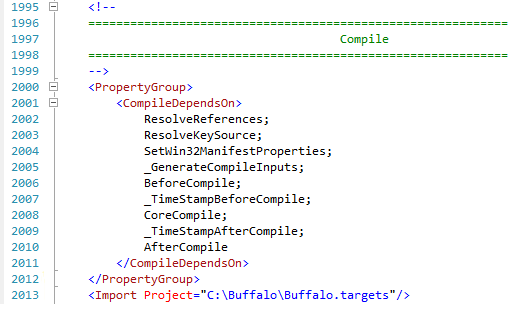
\includegraphics[scale=1.0]{CommonTarget.PNG}
  \centering
  \caption{Adding Buffalo.targets\label{buffalo_targets}}
\end{figure}

If you open Buffalo.targets in a text editor, it contains the following context:

\begin{lstlisting}[caption={Buffalo.targets}, label=buffalotargets, frame=tb, basicstyle=\scriptsize]
<Project xmlns="http://schemas.microsoft.com/developer/msbuild/2003">
  <PropertyGroup>
    <CompileDependsOn>
      $(CompileDependsOn);
      Buffalo
    </CompileDependsOn>
  </PropertyGroup>

  <Target Name="Buffalo">
    <Message Text="Hello Buffalo! @(IntermediateAssembly)"/>
    <Exec Command="&quot;C:\Buffalo\BuffaloAOP.exe&quot; &quot;@(IntermediateAssembly)&quot;"/>
  </Target>
</Project>
\end{lstlisting}

This is how Buffalo get hooked into MS-Build, what this mean is that when user compiles a project, everything defined in the CompileDependsOn property group will be performed first, then a new target named "Buffalo" will be called immediately, which will invoke the BuffaloAOP via the Exec Command. Note that for the Exec Command, a complete path to BuffaloAOP.exe must be provided, including the decoded quotation marks as shown.

Make sure to save all the changes. 

Now every time a C\# project is compiled, Buffalo will be invoked automatically to perform the weaving.
